Esta práctica se dividió en 3 diagramas pensando en la implementación, se realizó uno para las fechas en los 3 formatos dados, uno para las palabras clave (el cual se verá que es bastante simple) y uno para los números.

\section{Fechas}
Para las fechas se creo la siguiente expresión regular
	$$\boxed{dd\qty(-dd-dd|/dd/dd\qty(\varepsilon |dd))}$$
Dado esto, se creo el AFND con la siguiente tabla de transiciones

%\begin{table}[H]
%\centering
\begin{longtable}{||c||cccc||c||}
\hline
\hline
Etiqueta & d  & -  & /  & $\varepsilon$ & Tipo de Estado \\
\hline
\hline
1  & 2  & 0  & 0  & 1       & INICIO      \\
2  & 0  & 0  & 0  & 2,3     &             \\
3  & 4  & 0  & 0  & 3       &             \\
4  & 0  & 0  & 0  & 4,5     &             \\
5  & 0  & 6  & 17 & 5       &             \\
6  & 0  & 0  & 0  & 6,7     &             \\
7  & 8  & 0  & 0  & 7       &             \\
8  & 0  & 0  & 0  & 8,9     &             \\
9  & 10 & 0  & 0  & 9       &             \\
10 & 0  & 0  & 0  & 10,11   &             \\
11 & 0  & 12 & 0  & 11      &             \\
12 & 0  & 0  & 0  & 12,13   &             \\
13 & 14 & 0  & 0  & 13      &             \\
14 & 0  & 0  & 0  & 14,15   &             \\
15 & 16 & 0  & 0  & 15      &             \\
16 & 0  & 0  & 0  & 16      & ACEPTACION  \\
17 & 0  & 0  & 0  & 17,18   &             \\
18 & 19 & 0  & 0  & 18      &             \\
19 & 0  & 0  & 0  & 19,20   &             \\
20 & 21 & 0  & 0  & 20      &             \\
21 & 0  & 0  & 0  & 21,22   &             \\
22 & 0  & 0  & 23 & 22      &             \\
23 & 0  & 0  & 0  & 23,24   &             \\
24 & 25 & 0  & 0  & 24      &             \\
25 & 0  & 0  & 0  & 25,26   &             \\
26 & 27 & 0  & 0  & 26      &             \\
27 & 0  & 0  & 0  & 27,28   & ACEPTACION  \\
28 & 29 & 0  & 0  & 28      &             \\
29 & 0  & 0  & 0  & 29,30   &             \\
30 & 31 & 0  & 0  & 30      &             \\
31 & 0  & 0  & 0  & 31      & ACEPTACION  \\
\hline
\hline

\caption{Tabla de la Función de Transición AFND}
\label{AFNDFechas}
\end{longtable}
%\end{table}

Con esto, se construyó la tabla de transiciones del AFD deseado, esta se muestra a continuación

%\begin{table}
%\centering
\begin{longtable}{||c|c||ccc||c||}
\hline
\hline
Numeración AFD & Elemento de \$\textbackslash{}mathcal\{P\} (Q)\$ & d  & -  & /  & Tipo de Estado  \\
\hline
\hline
0              & 1                                                & 2  & 0  & 0  & INICIO          \\
1              & 2                                                & 4  & 0  & 0  &                 \\
2              & 4                                                & 0  & 6  & 17 &                 \\
3              & 6                                                & 8  & 0  & 0  &                 \\
4              & 17                                               & 19 & 0  & 0  &                 \\
5              & 19                                               & 21 & 0  & 0  &                 \\
6              & 21                                               & 0  & 0  & 23 &                 \\
7              & 23                                               & 25 & 0  & 0  &                 \\
8              & 25                                               & 27 & 0  & 0  &                 \\
9              & 27                                               & 29 & 0  & 0  & ACEPTACION      \\
10             & 29                                               & 31 & 0  & 0  &                 \\
11             & 31                                               & 0  & 0  & 0  & ACEPTACION      \\
12             & 8                                                & 10 & 0  & 0  &                 \\
13             & 10                                               & 0  & 12 & 0  &                 \\
14             & 12                                               & 14 & 0  & 0  &                 \\
15             & 14                                               & 16 & 0  & 0  &                 \\
16             & 16                                               & 0  & 0  & 0  & ACEPTACION      \\
\hline
\hline

\caption{Tabla de Transiciones AFD}
\label{AFDfechas}
\end{longtable}
%\end{table}

Dada esta tabla, se construyó el siguiente AFD

\begin{figure}[H]
	\centering
	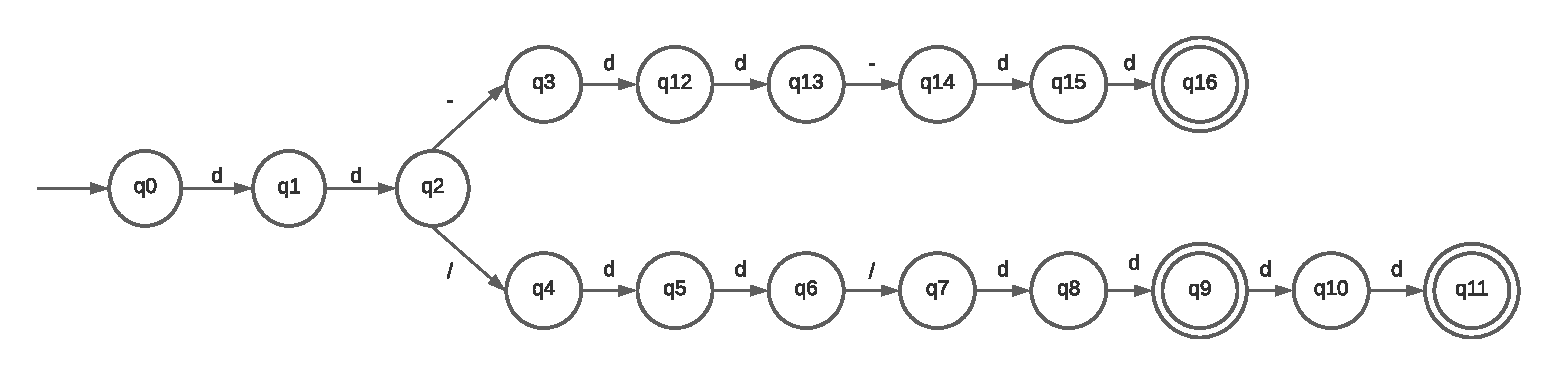
\includegraphics[scale=0.6]{Images/fechas.pdf}
	\caption{AFD para reconocimiento de fechas en dos formatos distintos.}
\end{figure}

\section{Parabras Clave}
Para las palabras clave simplemente se generó un conjunto que las contiene ($P$) y una expresión regular simple 
	$$\boxed{P}.$$
De modo que el AFD es el de un único estado.
\section{Números}
Para los números enteros, reales, complejos y en notación científica, se creó una expresión regular que acepte cualquier forma de dichos números. Los de notación científica tienen que estar específicamente en el formato de "exp" y luego del "exp" solo acepta un número entero.

\begin{align*}
	&(\varepsilon | -) dd* \left(\varepsilon \Bigg| i \Bigg| .dd* \qty(\varepsilon \Bigg| i\Bigg| exp(\varepsilon | -)dd*(\varepsilon | i) \Bigg| (+|-)dd* \qty(i \Big| .dd* \qty(i \Big| exp (\varepsilon | -) dd*i) \Big| exp (\varepsilon | -) dd* i )) \right. \Bigg| \\
	&\left. exp (\varepsilon | -)dd*\qty( \varepsilon \Bigg| i \Bigg| (+|-) dd* \qty(i \Big| .dd* \qty(i \Big| exp (\varepsilon | -) dd* i) \Bigg| exp (\varepsilon | -)dd* i) )  \right) .
\end{align*}

Con esta expresión es fácil ver que acepta cualquier número en el formato dado anteriormente, tanto reales puros, como complejos compuestos y puros. \\

Para crear el autómata se uso el método de Thompson, convertimos esta ER a un AFND. Dado que el autómata tiene un conjunto de estados superior a 100, únicamente se mostrará la tabla de transiciones de dicho AFND (los $0$s representan el vacío.)
%\pagebreak
%\begin{table}[H]
%\centering
\begin{longtable}{||c||ccccccc||c||}
\hline
\hline
Etiqueta & d   & .  & +  & -   & exp & i   & $\varepsilon$           & Tipo de Estado \\
\hline
\hline
1   & 0   & 0  & 0  & 0   & 0   & 0   & 1,2,3,4,6               & INICIO      \\
2   & 0   & 0  & 0  & 0   & 0   & 0   & 2,4,6                   &             \\
3   & 0   & 0  & 0  & 5   & 0   & 0   & 3                       &             \\
4   & 0   & 0  & 0  & 0   & 0   & 0   & 4,6                     &             \\
5   & 0   & 0  & 0  & 0   & 0   & 0   & 5,6                     &             \\
6   & 7   & 0  & 0  & 0   & 0   & 0   & 6                       &             \\
7   & 0   & 0  & 0  & 0   & 0   & 0   & 6,7,8,59,61             & ACEPTACION  \\
8   & 0   & 9  & 0  & 0   & 0   & 0   & 8                       &             \\
9   & 0   & 0  & 0  & 0   & 0   & 0   & 9,10                    &             \\
10  & 11  & 0  & 0  & 0   & 0   & 0   & 10                      &             \\
11  & 0   & 0  & 0  & 0   & 0   & 0   & 10,11,12,14,24,25,26,49 & ACEPTACION  \\
12  & 0   & 0  & 0  & 0   & 0   & 13  & 12                      &             \\
13  & 0   & 0  & 0  & 0   & 0   & 0   & 13                      & ACEPTACION  \\
14  & 0   & 0  & 0  & 0   & 15  & 0   & 14                      &             \\
15  & 0   & 0  & 0  & 0   & 0   & 0   & 15,16,17,18,20          &             \\
16  & 0   & 0  & 0  & 0   & 0   & 0   & 16,18,20                &             \\
17  & 0   & 0  & 0  & 19  & 0   & 0   & 17                      &             \\
18  & 0   & 0  & 0  & 0   & 0   & 0   & 18,20                   &             \\
19  & 0   & 0  & 0  & 0   & 0   & 0   & 19,20                   &             \\
20  & 21  & 0  & 0  & 0   & 0   & 0   & 20                      &             \\
21  & 0   & 0  & 0  & 0   & 0   & 0   & 20,21,22                & ACEPTACION  \\
22  & 0   & 0  & 0  & 0   & 0   & 23  & 22                      &             \\
23  & 0   & 0  & 0  & 0   & 0   & 0   & 23                      & ACEPTACION  \\
24  & 0   & 0  & 0  & 0   & 0   & 0   & 24,25,26                &             \\
25  & 0   & 0  & 27 & 0   & 0   & 0   & 25                      &             \\
26  & 0   & 0  & 0  & 28  & 0   & 0   & 26                      &             \\
27  & 0   & 0  & 0  & 0   & 0   & 0   & 27,29                   &             \\
28  & 0   & 0  & 0  & 0   & 0   & 0   & 28,29                   &             \\
29  & 30  & 0  & 0  & 0   & 0   & 0   & 29                      &             \\
30  & 0   & 0  & 0  & 0   & 0   & 0   & 29,30,31,33             &             \\
31  & 0   & 0  & 0  & 0   & 0   & 32  & 31                      &             \\
32  & 0   & 0  & 0  & 0   & 0   & 0   & 32                      & ACEPTACION  \\
33  & 0   & 34 & 0  & 0   & 0   & 0   & 33                      &             \\
34  & 0   & 0  & 0  & 0   & 0   & 0   & 34,35                   &             \\
35  & 36  & 0  & 0  & 0   & 0   & 0   & 35                      &             \\
36  & 0   & 0  & 0  & 0   & 0   & 0   & 35,36,37,39             &             \\
37  & 0   & 0  & 0  & 0   & 0   & 38  & 37                      &             \\
38  & 0   & 0  & 0  & 0   & 0   & 0   & 38                      & ACEPTACION  \\
39  & 0   & 0  & 0  & 0   & 40  & 0   & 39                      &             \\
40  & 0   & 0  & 0  & 0   & 0   & 0   & 40,41,42,43,45          &             \\
41  & 0   & 0  & 0  & 44  & 0   & 0   & 41                      &             \\
42  & 0   & 0  & 0  & 0   & 0   & 0   & 42,43,45                &             \\
43  & 0   & 0  & 0  & 0   & 0   & 0   & 43,45                   &             \\
44  & 0   & 0  & 0  & 0   & 0   & 0   & 44,45                   &             \\
45  & 46  & 0  & 0  & 0   & 0   & 0   & 45                      &             \\
46  & 0   & 0  & 0  & 0   & 0   & 0   & 45,46,47                &             \\
47  & 0   & 0  & 0  & 0   & 0   & 48  & 47                      &             \\
48  & 0   & 0  & 0  & 0   & 0   & 0   & 48                      & ACEPTACION  \\
49  & 0   & 0  & 0  & 0   & 50  & 0   & 49                      &             \\
50  & 0   & 0  & 0  & 0   & 0   & 0   & 50,51,52,53,55          &             \\
51  & 0   & 0  & 0  & 0   & 0   & 0   & 51,53,55                &             \\
52  & 0   & 0  & 0  & 54  & 0   & 0   & 52                      &             \\
53  & 0   & 0  & 0  & 0   & 0   & 0   & 53,55                   &             \\
54  & 0   & 0  & 0  & 0   & 0   & 0   & 54,55                   &             \\
55  & 56  & 0  & 0  & 0   & 0   & 0   & 55                      &             \\
56  & 0   & 0  & 0  & 0   & 0   & 0   & 55,56,57                &             \\
57  & 0   & 0  & 0  & 0   & 0   & 58  & 57                      &             \\
58  & 0   & 0  & 0  & 0   & 0   & 0   & 58                      & ACEPTACION  \\
59  & 0   & 0  & 0  & 0   & 0   & 60  & 59                      &             \\
60  & 0   & 0  & 0  & 0   & 0   & 0   & 60                      & ACEPTACION  \\
61  & 0   & 0  & 0  & 0   & 62  & 0   & 61                      &             \\
62  & 0   & 0  & 0  & 0   & 0   & 0   & 62,63,64,66,67          &             \\
63  & 0   & 0  & 0  & 65  & 0   & 0   & 63                      &             \\
64  & 0   & 0  & 0  & 0   & 0   & 0   & 64,66,67                &             \\
65  & 0   & 0  & 0  & 0   & 0   & 0   & 65,67                   &             \\
66  & 0   & 0  & 0  & 0   & 0   & 0   & 66,67                   &             \\
67  & 68  & 0  & 0  & 0   & 0   & 0   & 67                      &             \\
68  & 0   & 0  & 0  & 0   & 0   & 0   & 67,68,69,71,72,73       & ACEPTACION  \\
69  & 0   & 0  & 0  & 0   & 0   & 70  & 69                      &             \\
70  & 0   & 0  & 0  & 0   & 0   & 0   & 70                      & ACEPTACION  \\
71  & 0   & 0  & 0  & 0   & 0   & 0   & 71,72,73                &             \\
72  & 0   & 0  & 0  & 75  & 0   & 0   & 72                      &             \\
73  & 0   & 0  & 74 & 0   & 0   & 0   & 73                      &             \\
74  & 0   & 0  & 0  & 0   & 0   & 0   & 74,76                   &             \\
75  & 0   & 0  & 0  & 0   & 0   & 0   & 75,76                   &             \\
76  & 77  & 0  & 0  & 0   & 0   & 0   & 76                      &             \\
77  & 0   & 0  & 0  & 0   & 0   & 0   & 77,78,80,96             &             \\
78  & 0   & 0  & 0  & 0   & 0   & 79  & 78                      &             \\
79  & 0   & 0  & 0  & 0   & 0   & 0   & 79                      & ACEPTACION  \\
80  & 0   & 81 & 0  & 0   & 0   & 0   & 80                      &             \\
81  & 0   & 0  & 0  & 0   & 0   & 0   & 81,82                   &             \\
82  & 83  & 0  & 0  & 0   & 0   & 0   & 82                      &             \\
83  & 0   & 0  & 0  & 0   & 0   & 0   & 82,83,84,85             &             \\
84  & 0   & 0  & 0  & 0   & 87  & 0   & 84                      &             \\
85  & 0   & 0  & 0  & 0   & 0   & 86  & 85                      &             \\
86  & 0   & 0  & 0  & 0   & 0   & 0   & 86                      & ACEPTACION  \\
87  & 0   & 0  & 0  & 0   & 0   & 0   & 87,88,89,91,92          &             \\
88  & 0   & 0  & 0  & 90  & 0   & 0   & 88                      &             \\
89  & 0   & 0  & 0  & 0   & 0   & 0   & 89,91,92                &             \\
90  & 0   & 0  & 0  & 0   & 0   & 0   & 90,92                   &             \\
91  & 0   & 0  & 0  & 0   & 0   & 0   & 91,92                   &             \\
92  & 93  & 0  & 0  & 0   & 0   & 0   & 92                      &             \\
93  & 0   & 0  & 0  & 0   & 0   & 0   & 92,93,94                &             \\
94  & 0   & 0  & 0  & 0   & 0   & 95  & 94                      &             \\
95  & 0   & 0  & 0  & 0   & 0   & 0   & 95                      & ACEPTACION  \\
96  & 0   & 0  & 0  & 0   & 97  & 0   & 96                      &             \\
97  & 0   & 0  & 0  & 0   & 0   & 0   & 97,98,99,101,102        &             \\
98  & 0   & 0  & 0  & 100 & 0   & 0   & 98                      &             \\
99  & 0   & 0  & 0  & 0   & 0   & 0   & 99,101,102              &             \\
100 & 0   & 0  & 0  & 0   & 0   & 0   & 100,102                 &             \\
101 & 0   & 0  & 0  & 0   & 0   & 0   & 101,102                 &             \\
102 & 103 & 0  & 0  & 0   & 0   & 0   & 102                     &             \\
103 & 0   & 0  & 0  & 0   & 0   & 0   & 102,103,104             &             \\
104 & 0   & 0  & 0  & 0   & 0   & 105 & 104                     &             \\
105 & 0   & 0  & 0  & 0   & 0   & 0   & 105                     & ACEPTACION  \\
\hline
\hline

\caption{Tabla de la Función de Transición AFND}
\label{AFNDnumeros}
\end{longtable}
%\end{table}


Dado esto, se transformó a un AFD con la siguiente tabla de estados


%\begin{table}
%\centering
\begin{longtable}{||c|c||cccccc||c||}
\hline
\hline
AFD Numeración & Elemento de $\mathcal{P} (Q)$ & d     & .  & +  & -     & exp   & i     & Tipo de Estado \\
\hline
\hline
1  & 1,2,3,4,6 & 7     & 0  & 0  & 5     & 0     & 0     & INICIO      \\
2  & 7         & 7     & 9  & 0  & 0     & 62    & 60    & ACEPTACION  \\
3  & 5         & 7     & 0  & 0  & 0     & 0     & 0     &             \\
4  & 9         & 11    & 0  & 0  & 0     & 0     & 0     &             \\
5  & 11        & 11    & 0  & 27 & 28    & 15,50 & 13    & ACEPTACION  \\
6  & 13        & 0     & 0  & 0  & 0     & 0     & 0     & ACEPTACION  \\
7  & 15,50     & 21,56 & 0  & 0  & 19,54 & 0     & 0     &             \\
8  & 27        & 30    & 0  & 0  & 0     & 0     & 0     &             \\
9  & 28        & 30    & 0  & 0  & 0     & 0     & 0     &             \\
10 & 21,56     & 21,56 & 0  & 0  & 0     & 0     & 23,58 & ACEPTACION  \\
11 & 19,54     & 21,56 & 0  & 0  & 0     & 0     & 0     &             \\
12 & 30        & 30    & 34 & 0  & 0     & 0     & 32    &             \\
13 & 23,58     & 0     & 0  & 0  & 0     & 0     & 0     & ACEPTACION  \\
14 & 32        & 0     & 0  & 0  & 0     & 0     & 0     & ACEPTACION  \\
15 & 34        & 36    & 0  & 0  & 0     & 0     & 0     &             \\
16 & 36        & 36    & 0  & 0  & 0     & 40    & 38    &             \\
17 & 38        & 0     & 0  & 0  & 0     & 0     & 0     & ACEPTACION  \\
18 & 40        & 46    & 0  & 0  & 44    & 0     & 0     &             \\
19 & 44        & 46    & 0  & 0  & 0     & 0     & 0     &             \\
20 & 46        & 46    & 0  & 0  & 0     & 0     & 48    &             \\
21 & 48        & 0     & 0  & 0  & 0     & 0     & 0     & ACEPTACION  \\
22 & 60        & 0     & 0  & 0  & 0     & 0     & 0     & ACEPTACION  \\
23 & 62        & 68    & 0  & 0  & 65    & 0     & 0     &             \\
24 & 65        & 68    & 0  & 0  & 0     & 0     & 0     &             \\
25 & 68        & 68    & 0  & 74 & 75    & 0     & 70    & ACEPTACION  \\
26 & 70        & 0     & 0  & 0  & 0     & 0     & 0     & ACEPTACION  \\
27 & 74        & 77    & 0  & 0  & 0     & 0     & 0     &             \\
28 & 75        & 77    & 0  & 0  & 0     & 0     & 0     &             \\
29 & 77        & 0     & 81 & 0  & 0     & 97    & 79    &             \\
30 & 79        & 0     & 0  & 0  & 0     & 0     & 0     & ACEPTACION  \\
31 & 81        & 83    & 0  & 0  & 0     & 0     & 0     &             \\
32 & 83        & 83    & 0  & 0  & 0     & 87    & 86    &             \\
33 & 86        & 0     & 0  & 0  & 0     & 0     & 0     & ACEPTACION  \\
34 & 87        & 93    & 0  & 0  & 90    & 0     & 0     &             \\
35 & 90        & 93    & 0  & 0  & 0     & 0     & 0     &             \\
36 & 93        & 93    & 0  & 0  & 0     & 0     & 95    &             \\
37 & 95        & 0     & 0  & 0  & 0     & 0     & 0     & ACEPTACION  \\
38 & 97        & 103   & 0  & 0  & 100   & 0     & 0     &             \\
39 & 100       & 103   & 0  & 0  & 0     & 0     & 0     &             \\
40 & 103       & 103   & 0  & 0  & 0     & 0     & 105   &             \\
41 & 105       & 0     & 0  & 0  & 0     & 0     & 0     & ACEPTACION  \\
\hline
\hline

\caption{Tabla de la Función de Transición AFD}
\label{AFDnumeros}
\end{longtable}
%\end{table}


Con todo esto, se llegó a la forma visual del autómata, la cual se inició en el software en el cual se hizo la de las fechas, pero por restricciones del programa hay número limitado de objetos, entonces se hizo a mano y se adjuntó una foto del mismo.










%%%%%%